Autonomous systems, in some form, have been imagined and realized for the bulk of recorded history. In ancient Greek mythology, the god Hephaestus, the `patron of invention and technology' \citep{MayorGodsRobots2019} was said to create talking mechanical hand-maidens, while early Hindu and Buddhist texts tell of \textit{yantakara} that lived in Greece and created machines that helped in trade and farming. The secret methods of the \textit{yantakara} (the early `roboticists') were closely guarded, and mechanical assassins were said to pursue and kill any person who revealed their techniques\footnote{Please be careful distributing this thesis.} \citep{MayorGodsRobots2019}.
 
%https://scroll.in/article/916490/in-an-ancient-indian-legend-robots-guarded-buddhas-relics
%Cite 

\begin{wrapfigure}{r}{0.5\textwidth}
  \begin{center}
  	\vspace{-20pt}
    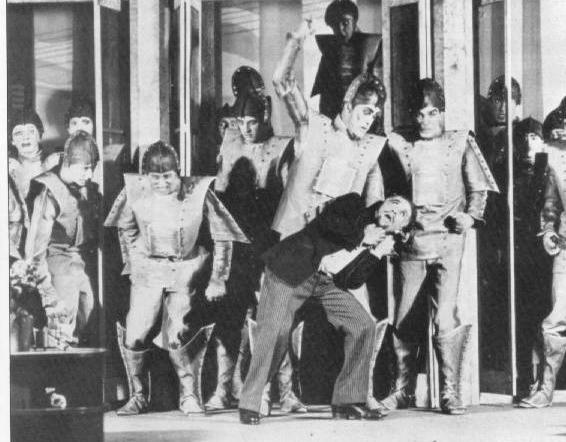
\includegraphics[width=0.4\textwidth]{introduction/rur.jpg}
     \vspace{-15pt}
  \end{center}
  \caption{A `robot' rebellion from Karel Capek's 1920 play, \textit{Rossum's Universal Robots}.}
  \vspace{-5pt}
  \label{fig:into_rur}
\end{wrapfigure}

Since the industrial revolution, the idea of an autonomous machine--one that requires no, or very minimal, human intervention or oversight to operate--has been imagined in different ways. Depending on one's perspective, autonomous machines have perennially promised to either usher in a utopia of freedom, or threatened to bring about an age of job loss and social upheaval that worsens socioeconomic divisions. Much like the Luddites of the 19th century, the social critics of the 21st century have continued the dialectic to understand the social ramifications of modern \textit{yantakara} and their newly-created autonomous hand-maidens.

These controversial origins are embedded even within the modern name of for the academic field, \textit{robotics}. The word \textit{robot} comes from the title of a science fiction play, R.U.R.: Rossum's Universal Robots, written by the Czech playwright Karel Capek in 1920 (see \Cref{fig:into_rur}). In naming the play, the word \textit{robot} was derived from the Slavic term for slave, \textit{rab}, and its Czech derivative for serf labour, \textit{rabota}, while the name \textit{Rossum} was inspired by the Czech word for reason, or intellect. Indeed, the concept of enslaved or embodied  intelligence is at the heart of modern definitions of the discipline of robotics \citep{Redfield2019-pi}. Much of the popular culture surrounding robots (e.g., Shelley's \textit{Frankenstein}, Asimov's \textit{I, Robot}, Kubrick's and Clarke's \textit{2001: A Space Odyssey}) also paints a complicated picture of humanity's relationship with such enslaved machines. In this dissertation, we focus on improving a specific part of a modern mobile \textit{autonomy} pipeline, while minimizing the use of term \textit{robot} to avoid the maelstrom of philosophical and ethical problems that it connotes. We hope this work aids the march of technological progress towards a future which finds some Hegelian synthesis of autonomy and humanity---a future in which human-in-the-loop autonomous systems augment and improve the lot of many people while still negotiating and constantly considering the social costs that come with technological innovation.
